\documentclass[sigconf,authordraft]{acmart}

\AtBeginDocument{%
  \providecommand\BibTeX{{%
    Bib\TeX}}}

% Draft-friendly ACM settings.
% Replace these metadata fields later when you know the target venue.
\setcopyright{none}
\settopmatter{printacmref=false}
\renewcommand\footnotetextcopyrightpermission[1]{}
\pagestyle{plain}

\acmConference[FMoE Draft]{Draft Venue Placeholder}{2026}{TBD}
\acmBooktitle{Draft Template for FMoE Paper}
\acmDOI{}
\acmISBN{}

% ------------------------------------------------------------------
% Notes for future editing
% ------------------------------------------------------------------
% Figure example:
% \begin{figure}[t]
%   \centering
%   \includegraphics[width=\linewidth]{figures/overview.pdf}
%   \caption{Overall framework of FMoE.}
%   \label{fig:overview}
% \end{figure}
%
% Bibliography example:
% 1) Create refs.bib in the same project folder.
% 2) Add entries there.
% 3) Uncomment the bibliography commands at the end of this file.

\begin{document}

\title[FeaturedMoE for Sequential Recommendation]{FeaturedMoE: Feature-Guided Mixture-of-Experts for Sequential Recommendation}

\author{First Author}
\affiliation{%
  \institution{KAIST}
  \department{Kim Jaechul Graduate School of AI}
  \city{Daejeon}
  \country{Republic of Korea}}
\email{first.author@kaist.ac.kr}

\author{Second Author}
\affiliation{%
  \institution{KAIST}
  \department{Kim Jaechul Graduate School of AI}
  \city{Daejeon}
  \country{Republic of Korea}}
\email{second.author@kaist.ac.kr}

\renewcommand{\shortauthors}{Author et al.}

\begin{abstract}
Mixture-of-experts (MoE) architectures are increasingly used in sequential recommendation because they can allocate different computation paths to different behavioral patterns. In many existing models, however, routing is still driven mainly by hidden states, so expert assignment remains difficult to interpret and verify. At the same time, feature-aware recommenders usually use side information to enrich representations rather than to guide the computation path itself. We propose FeaturedMoE (FMoE), a feature-guided modular architecture that bridges these two directions. FMoE derives compact behavioral cues from raw signals that are widely available in sequential recommendation data---sessionized interaction order, timestamps, and item categories---and uses them to guide macro, mid, and micro routing stages. Instead of relying on a large handcrafted feature bank or rich dataset-specific metadata, FMoE organizes these cues into a small set of behavioral families that act as explicit routing signals. Our experiments show that compact multi-family features are sufficient to support effective routing, that stage composition materially affects performance, and that corrupted or semantically misaligned cues consistently degrade the model. These results suggest that common raw sequential signals can serve as practical and inspectable routing priors for MoE-based sequential recommendation.
\end{abstract}

% Add proper CCS terms later if needed for the final submission.
% \begin{CCSXML}
% ...
% \end{CCSXML}
% \ccsdesc[500]{...}

\keywords{sequential recommendation, mixture of experts, conditional computation, routing, behavioral features}

\maketitle


\section{Introduction}
Sequential recommendation aims to predict the next item from a temporally ordered interaction history. Although this task is usually written as next-item prediction, the behavior behind a sequence is rarely governed by a single homogeneous signal. Long-term preference, temporary session intent, and highly local transition patterns often coexist, interact, and change in strength over time. This view is well aligned with the broader understanding of sequential and session-based recommendation in prior surveys and benchmark literature~\cite{wang2019seqsurvey,wang2021sessionsurvey}.

A large body of sequential recommenders has focused on building stronger sequence encoders. Early neural models such as GRU4Rec, NARM, STAMP, SR-GNN, Caser, and NextItNet improved over classical Markov-style formulations by learning richer transition patterns from interaction sequences~\cite{hidasi2016gru4rec,li2017narm,liu2018stamp,wu2019srgnn,tang2018caser,yuan2019nextitnet}. Transformer-based models, especially SASRec and BERT4Rec, then became standard backbones for capturing long- and short-range dependencies with self-attention~\cite{kang2018sasrec,sun2019bert4rec}. Yet these models, despite their modeling strength, still process heterogeneous behavioral regimes through largely shared computation.

A second line of work enriches sequential models with additional signals or architectural biases. TiSASRec incorporates explicit time intervals into attention, FDSA models feature-level transitions, and DIF-SR revisits how side information should interact with attention~\cite{li2020tisasrec,zhang2019fdsa,xie2022difsr}. Self-supervised and contrastive approaches such as DSSRec, S$^3$-Rec, CL4SRec, Sequential Recommendation with Multiple Contrast Signals, and DuoRec improve representation quality by mining auxiliary supervisory signals or correcting representation degeneration~\cite{ma2020dssrec,zhou2020s3rec,xie2020cl4srec,wang2023multiplecontrast,qiu2022duorec}. Recent architectural alternatives including FMLP-Rec, FEARec, BSARec, and SIGMA study frequency bias, efficiency, or non-Transformer sequence modeling~\cite{zhou2022fmlprec,du2023fearec,shin2024bsarec,liu2025sigma}. These methods are important, but they are still mostly representation-centric: extra cues are typically used to strengthen hidden states, not to explicitly organize the computation path.

Mixture-of-experts (MoE) offers a natural way to introduce conditional computation~\cite{jacobs1991adaptive,jordan1994hme,shazeer2017moe}. In large-scale modeling, modern sparse MoE research has shown that routing design, expert utilization, and stabilization are central to whether specialization actually emerges~\cite{lepikhin2021gshard,fedus2022switch,du2022glam,zoph2022stmoe,zhou2022expertchoice,wang2024lossfree}. Recommendation has also adopted expert mixtures, most notably in multi-task settings such as MMoE and PLE~\cite{ma2018mmoe,tang2020ple}. For sequential recommendation, FAME is the clearest direct reference point: it introduces experts inside attention heads to disentangle facet-level preferences, while recent multimodal sequential recommenders such as M3SRec and HM4SR use expert mixtures mainly for modality fusion~\cite{liu2025fame,bian2023m3srec,zhang2025hm4sr}. However, routing in these models is not designed around a compact, explicitly interpretable set of behavioral cues derived from raw sequential logs.

We ask a different question: can a small set of portable behavioral cues organize expert routing in sequential recommendation? We propose FeaturedMoE (FMoE), a feature-guided mixture-of-experts framework built on top of a SASRec backbone. Instead of assuming rich dataset-specific metadata, FMoE derives compact routing cues from signals that are widely available in sequential logs---interaction order, timestamps, and coarse item categories---and instantiates them at three temporal scales: macro, mid, and micro. Rather than using these cues mainly to enrich item representations, FMoE uses them to decide which experts should process the hidden states at different temporal scopes.

Our contributions are threefold. First, we propose a compact behavioral feature bank that turns common raw sequential signals into explicit routing priors. Second, we design a stage-wise MoE structure in which macro, mid, and micro routing progressively move from coarse behavioral guidance to fine-grained local specialization. Third, we position FMoE against strong recurrent, attention-based, feature-aware, contrastive, frequency-aware, Mamba-based, and MoE-based baselines, and we explicitly evaluate stage composition, cue corruption, and routing diagnostics to test whether the learned specialization is meaningful rather than incidental.

\section{Related Work}
\label{sec:related}

\paragraph{Sequential recommendation backbones.}
Sequential recommendation has evolved from factorization- and recurrence-based formulations to increasingly expressive neural sequence encoders. FPMC combines matrix factorization with first-order Markov transitions~\cite{rendle2010fpmc}, while GRU4Rec established recurrent neural modeling for session-based recommendation~\cite{hidasi2016gru4rec}. NARM, STAMP, and SR-GNN subsequently emphasized session intent, short-term memory, and graph-structured transitions, respectively~\cite{li2017narm,liu2018stamp,wu2019srgnn}. CNN-based and dilated-convolution models such as Caser and NextItNet provided further alternatives~\cite{tang2018caser,yuan2019nextitnet}. Transformer-based models, especially SASRec and BERT4Rec, then became standard reference points for next-item recommendation~\cite{kang2018sasrec,sun2019bert4rec}. Recent alternatives such as FMLP-Rec and SIGMA revisit efficiency and backbone choice, but they still focus primarily on sequence encoding quality~\cite{zhou2022fmlprec,liu2025sigma}.

\paragraph{Structural bias, self-supervision, and representation regularization.}
A substantial line of work improves sequential recommenders by changing their inductive bias or training objective instead of changing the computation path. TiSASRec incorporates explicit time intervals into attention~\cite{li2020tisasrec}. FEARec and BSARec analyze self-attention from a frequency perspective and inject frequency-domain bias to alleviate the low-pass tendency of standard Transformers~\cite{du2023fearec,shin2024bsarec}. DSSRec and S$^3$-Rec introduce auxiliary self-supervision for future-intent and mutual-information-based pretraining~\cite{ma2020dssrec,zhou2020s3rec}. CL4SRec, Sequential Recommendation with Multiple Contrast Signals, and DuoRec further use contrastive learning to improve sequence representation quality and mitigate degeneration~\cite{xie2020cl4srec,wang2023multiplecontrast,qiu2022duorec}. These methods are highly relevant because they show that sequential recommendation benefits from additional structure, but the additional structure is usually applied to representation learning rather than routing.

\paragraph{Feature and side-information fusion.}
Another important direction studies how item attributes or side information should be incorporated into sequential models. FDSA explicitly models feature-level transition patterns in parallel with item-level transitions~\cite{zhang2019fdsa}. DIF-SR argues that naively fusing side information at the input level can limit attention expressiveness, and therefore moves side information into a decoupled attention computation~\cite{xie2022difsr}. Multimodal sequential recommendation extends this direction further by integrating text and image signals, with examples including M3SRec and HM4SR~\cite{bian2023m3srec,zhang2025hm4sr}. Unlike these approaches, we do not aim to maximize metadata coverage. Instead, we ask whether a small set of portable cues extracted from raw order, time, and category signals can serve as explicit routing priors.

\paragraph{Mixture-of-experts and routing stabilization.}
The classical MoE view goes back to adaptive mixtures of local experts and hierarchical mixtures of experts, where a gating network partitions the input space and delegates different regions to specialized experts~\cite{jacobs1991adaptive,jordan1994hme}. Modern sparse MoE reinterprets this idea as conditional computation at scale, with milestones including sparsely-gated MoE, GShard, Switch Transformer, GLaM, ST-MoE, and Expert Choice Routing~\cite{shazeer2017moe,lepikhin2021gshard,fedus2022switch,du2022glam,zoph2022stmoe,zhou2022expertchoice}. More recent work also examines routing stabilization directly, for example through auxiliary-loss-free balancing~\cite{wang2024lossfree}. These studies motivate our focus on routing semantics, collapse prevention, and stable specialization, even though they are not specific to sequential recommendation.

\paragraph{MoE in recommendation and sequential recommendation.}
MoE has already been influential in recommendation, especially in multi-task or multi-objective settings. MMoE and PLE are representative examples showing how gated experts can separate related but non-identical signals in recommendation pipelines~\cite{ma2018mmoe,tang2020ple}. For sequential recommendation, FAME is the most direct comparison to our work: it introduces expert mixtures inside attention heads to disentangle facet-level preferences~\cite{liu2025fame}. Multimodal sequential recommenders such as M3SRec and HM4SR also use expert mixtures, but mainly to coordinate modality-specific information~\cite{bian2023m3srec,zhang2025hm4sr}. In contrast, FMoE is centered on stage-wise behavioral routing: it uses compact cues from raw sequential logs to decide how computation should be specialized across temporal scopes.

\section{Methodology}
\label{sec:method}

\subsection{Problem Definition and Overall Framework}
\label{sec:problem-framework}

Sequential recommendation aims to predict the next item a user will interact with from the user's past behavior sequence. In our setting, the interaction history is organized into sessions, where a session denotes a contiguous period of activity corresponding to a coherent visit or intent. For readability, we omit the user index and describe the history of a single user. Let $\mathcal{S} = [s_1, \dots, s_M]$ denote the session sequence, where the $m$-th session is written as $s_m = [x_1, \dots, x_{|s_m|}]$. Each interaction $x_t$ contains an item ID and timestamp, and each item may additionally be associated with a category label. Given the observed interaction history, the goal is to predict the next item.

FMoE is built on top of a SASRec backbone~\cite{kang2018sasrec}. The backbone itself remains intentionally simple: the input structure is unchanged from standard sequential recommendation, and the main architectural change is the introduction of mixture-of-experts computation~\cite{jordan1994hme,shazeer2017moe,fedus2022switch}. The key idea is that expert routing is not driven only by hidden representations. Instead, FMoE constructs compact behavioral features from widely available raw sequential signals, such as sequence order, timestamps, and item categories, and uses them to guide expert selection. This preserves the strong sequence modeling capability of SASRec while introducing an explicit behavioral control signal into the computation path.

Let $\mathbf{h}_t$ denote the hidden state at position $t$, and let $\mathbf{f}_t$ denote the behavioral feature used for routing. The router produces expert weights $\boldsymbol{\pi}_t$, and the hidden representation is transformed by a weighted combination of experts:
\[
\tilde{\mathbf{h}}_t
=
\sum_{e=1}^{E}
\pi_{t,e}\,\mathrm{Expert}_e(\mathbf{h}_t).
\]
FMoE applies this routing mechanism at three behavioral levels---macro, mid, and micro---so that long-term tendency, session-level context, and immediate local transition can influence expert computation at different temporal scales. The next subsections describe how these behavioral features are constructed and how the stage-wise routers are designed.

\begin{figure*}[!t]
  \centering
  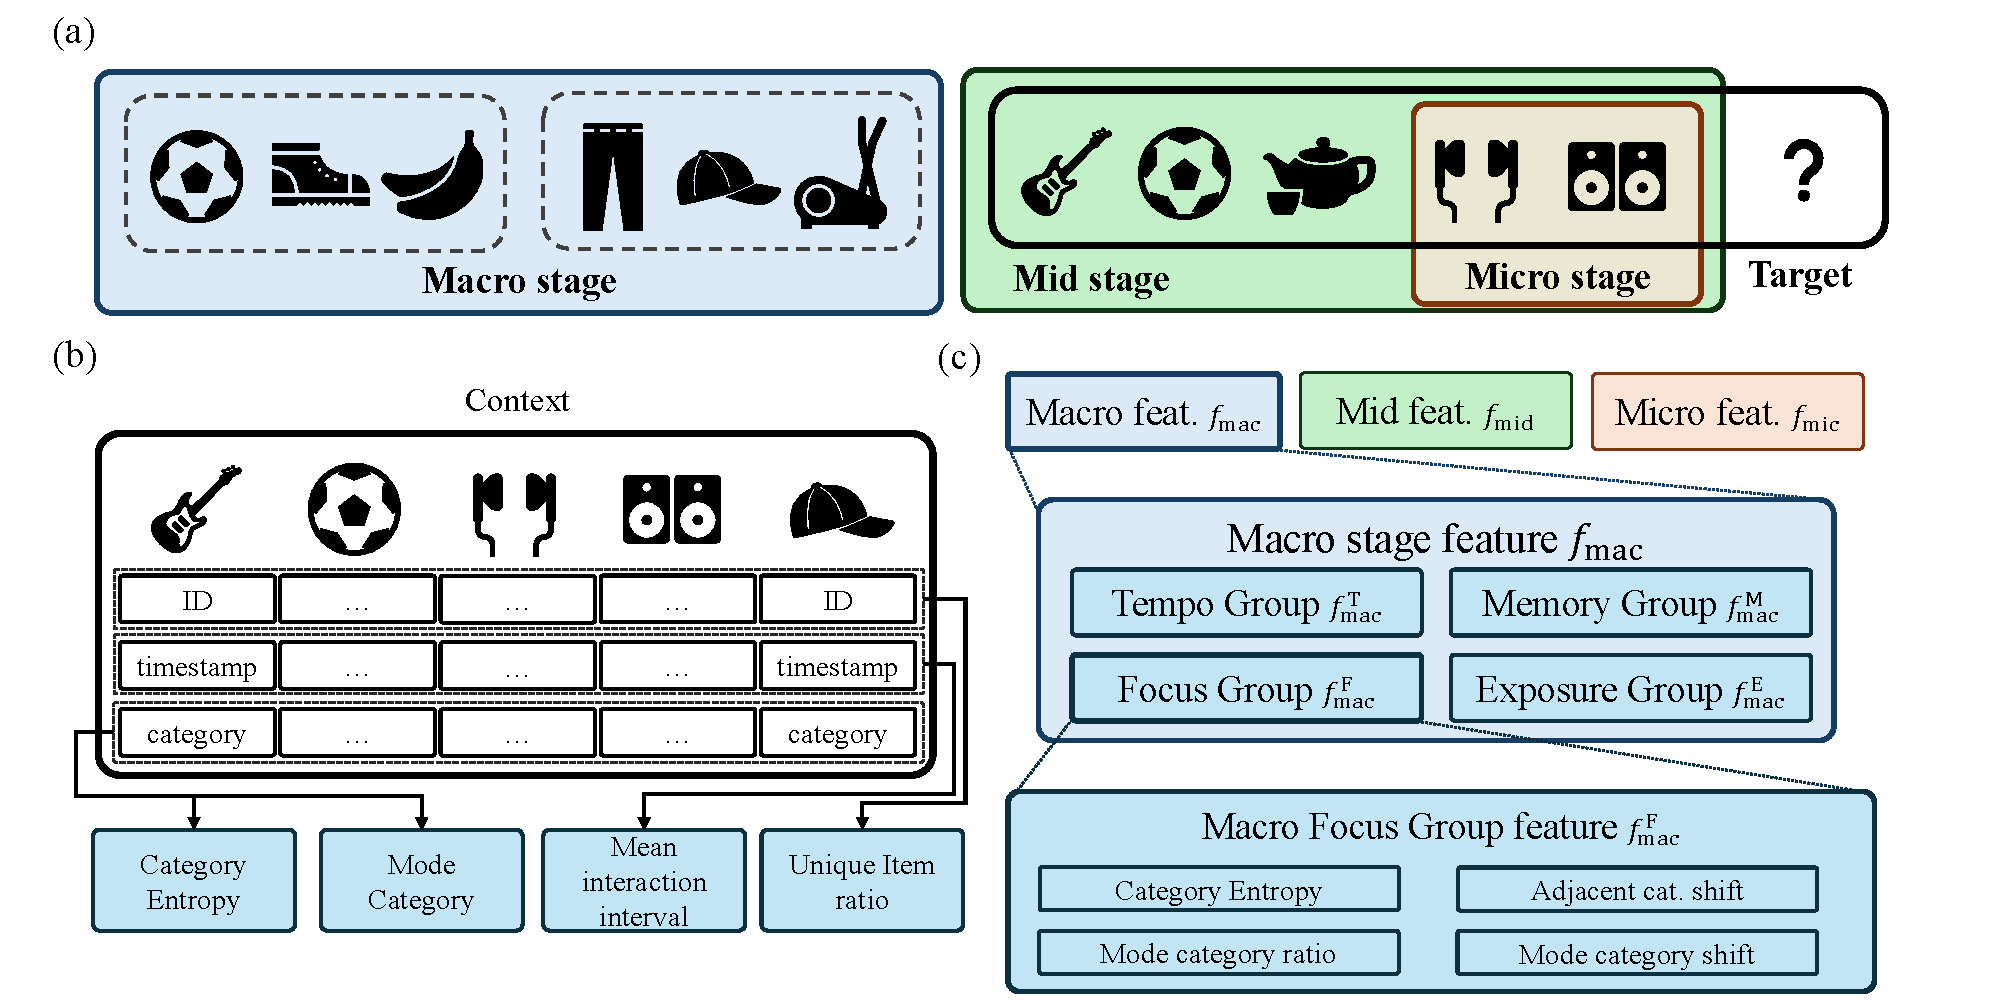
\includegraphics[width=0.94\textwidth]{figures/figure2_feature_construction.pdf}
  \caption{Behavioral feature construction in FMoE. (a) Stage-dependent observation scopes are defined around target position $t$: macro uses preceding sessions, mid uses the current-session prefix, and micro uses the most recent interactions. (b) Common raw signals such as interaction order, timestamps, and categories are converted into lightweight scalar descriptors within each scope. (c) The resulting stage feature is reorganized into shared behavioral groups (Tempo, Focus, Memory, and Exposure), while the scalar values remain stage-specific.}
  \label{fig:feature-construction}
\end{figure*}

\begin{figure*}[!t]
  \centering
  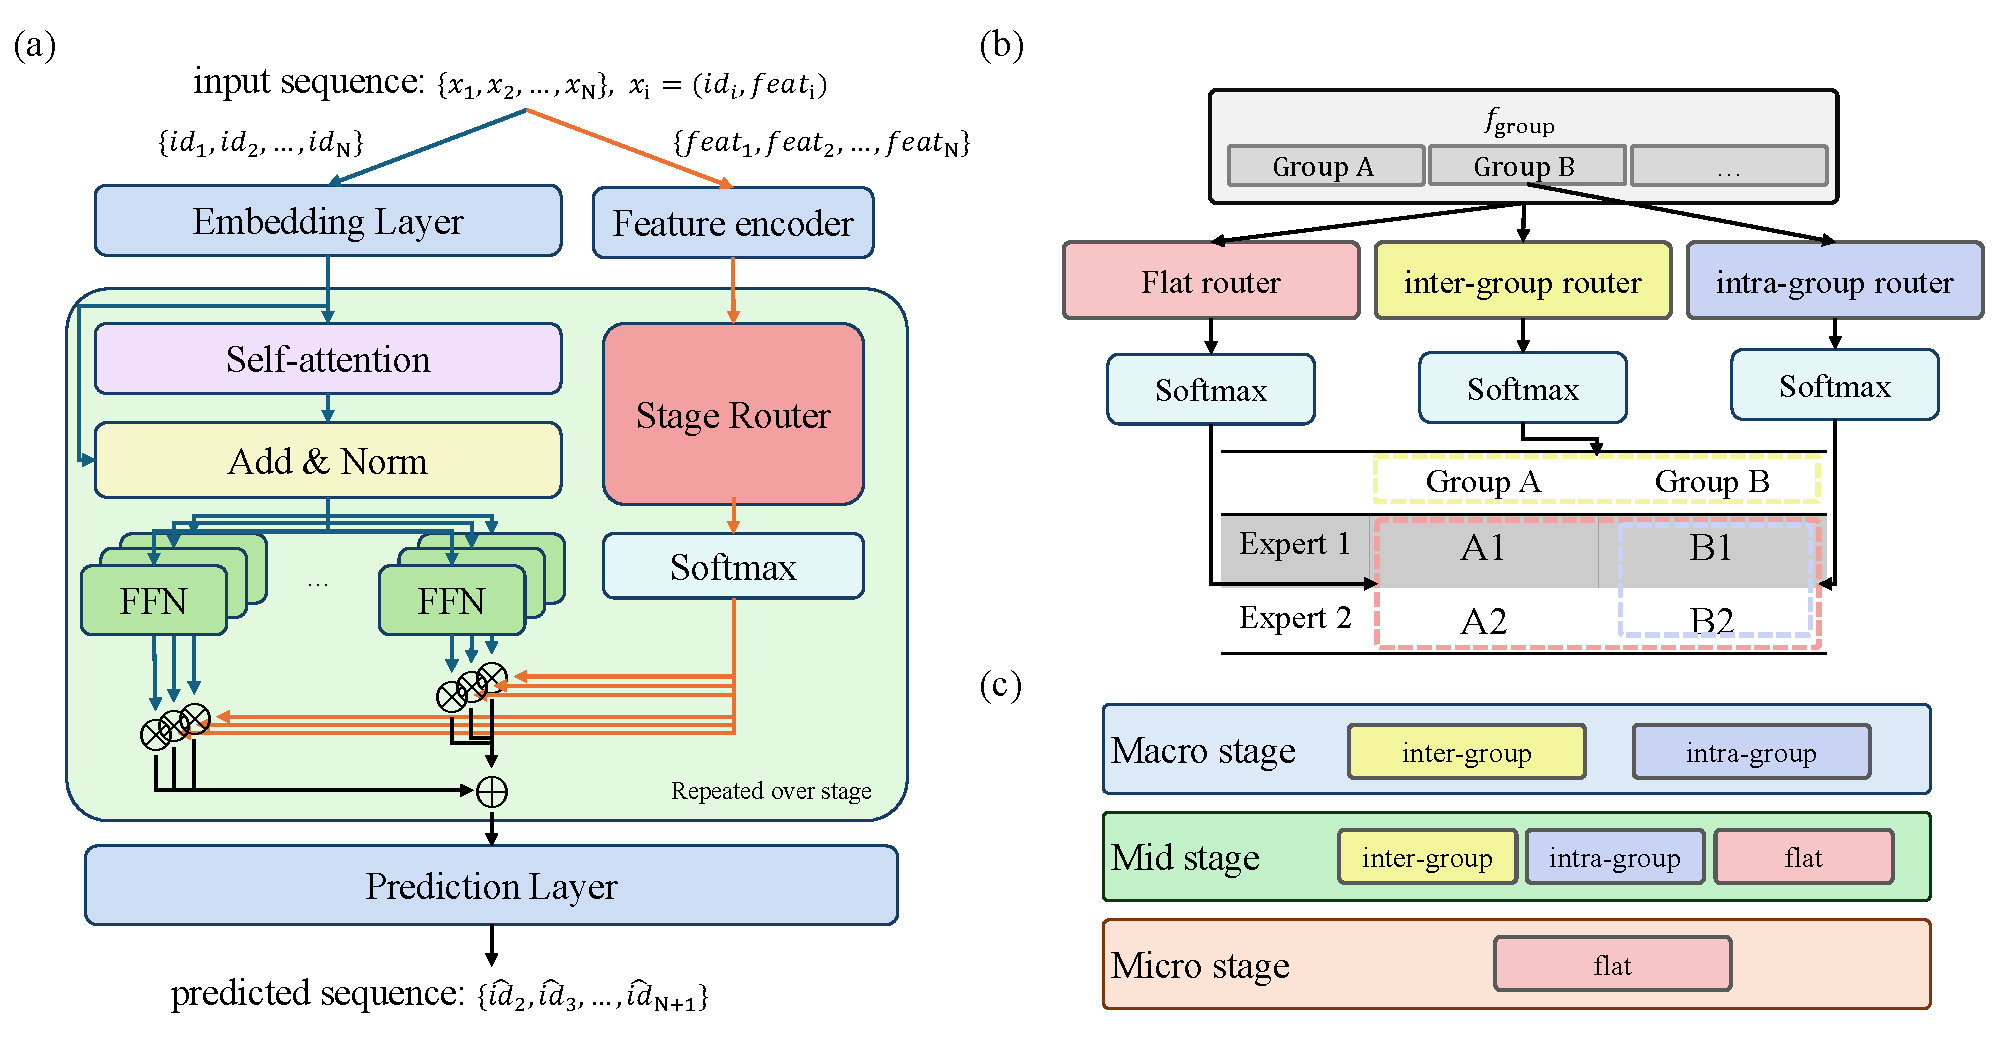
\includegraphics[width=0.94\textwidth]{figures/figure3_framwork.pdf}
  \caption{Feature-guided FMoE routing framework. (a) FMoE keeps the SASRec backbone and replaces shared feed-forward computation with stage-wise mixture-of-experts routing; in the A6 setting used in this paper, stage features alone determine routing weights, while expert FFNs transform the hidden states. (b) The routing module is decomposed into reusable primitives: \texttt{a\_joint} produces flat expert logits, \texttt{b\_group} produces group logits, and \texttt{d\_cond} produces group-conditional intra-group logits. (c) The three stages use different wrappers: macro uses $\log(b \times d)$, mid uses $\alpha_{\mathrm{struct}}\log(b \times d)+\alpha_a a$, and micro uses $a$ only.}
  \label{fig:framework}
\end{figure*}

\subsection{Behavioral Feature Construction from Raw Sequential Signals}
\label{sec:feature-construction}

Figure~\ref{fig:feature-construction} summarizes the feature-construction pipeline in three steps. Panel~(a) defines the stage-specific observation scopes around the same prediction target, panel~(b) shows how raw sequential metadata are converted into lightweight scalar descriptors, and panel~(c) shows how these descriptors are organized into a structured stage feature. Rather than enumerating every handcrafted statistic, this subsection focuses on how common raw signals become a compact routing-side feature bank with clear temporal semantics.

\subsubsection{Raw Signals and Scalar Summaries}

Starting from the notation in Section~\ref{sec:problem-framework}, recall that the current session is written as $s_m = [x_1, \dots, x_{|s_m|}]$. For each interaction $x_t$, FMoE uses only signals that are commonly available in sequential recommendation datasets: item identity $i_t$, timestamp $\tau_t$, and, when available, category label $c_t$. We additionally allow item-level popularity statistics computed from the training corpus. These inputs are deliberately simple. Instead of introducing a separate metadata encoder, FMoE converts them into low-dimensional scalar descriptors that can steer routing.

Figure~\ref{fig:feature-construction}(a) shows the three observation scopes defined around the same target position. The macro stage summarizes preceding sessions, the mid stage uses the current-session prefix, and the micro stage focuses on a short recent context immediately before the target. Figure~\ref{fig:feature-construction}(b) then illustrates how raw signals from a given scope are mapped to scalar descriptors, such as interval-, category-, or popularity-related summaries. The descriptor template is shared across stages, but its interpretation depends on the temporal range from which it is extracted.

Formally, let $\mathcal{R}$ denote an observation range and let
\[
\mathcal{A}(\mathcal{R}) = [a_1(\mathcal{R}), \dots, a_K(\mathcal{R})]
\]
be the vector of scalar summaries extracted from that range, where each $a_k(\cdot)$ is a lightweight aggregation such as a count, ratio, mean, entropy, or trend statistic. This notation is intentionally generic: the exact scalar list may vary across datasets, but the construction principle remains the same. FMoE does not assume a rich side-information schema; instead, it reconstructs routing cues from raw sequential evidence already present in standard interaction logs.

\subsubsection{Compact Feature Families}

The scalar summaries are not treated as an unstructured list. FMoE groups them into four behavioral families: \textit{Tempo}, \textit{Focus}, \textit{Memory}, and \textit{Exposure}. Tempo captures pace and interval patterns. Focus describes how concentrated behavior is around categories and how often the user switches among them. Memory reflects repetition, recurrence, and overlap with previously observed context. Exposure summarizes the popularity level of consumed items and its local drift.

This grouping step corresponds to Figure~\ref{fig:feature-construction}(c). The family definitions are shared across stages, but the actual scalar values differ because each stage observes a different temporal window. Let $\mathbf{f}$ denote a generic routing feature vector. We write it as
\[
\mathbf{f}
=
[\mathbf{f}^{\mathrm{tempo}} \,\|\, \mathbf{f}^{\mathrm{focus}} \,\|\, \mathbf{f}^{\mathrm{memory}} \,\|\, \mathbf{f}^{\mathrm{exposure}}],
\]
where each block corresponds to one behavioral family. This grouping is semantic rather than architectural: it presents the router with a structured view of behavior instead of a flat collection of unrelated statistics.

\subsubsection{Stage-Specific Feature Views}

The same four feature families are used at all stages, but they are computed over different observation ranges. Figure~\ref{fig:feature-construction}(a) visualizes these scopes around the same target position, while Figure~\ref{fig:feature-construction}(c) shows the shared group layout. With macro history window $H$ ($H=5$ in our main setting), the stage-dependent ranges are
\begin{align}
\mathcal{R}^{\mathrm{macro}} &= [s_{\max(1,m-H)}, \dots, s_{m-1}], \\
\mathcal{R}^{\mathrm{mid}}_t &= [x_1, \dots, x_{t-1}], \\
\mathcal{R}^{\mathrm{micro}}_t &= [x_{\max(1,t-5)}, \dots, x_{t-1}].
\end{align}
Applying the scalar-summary operator $\mathcal{A}(\cdot)$ to these ranges gives
\begin{align}
\mathbf{f}^{\mathrm{macro}} &= \mathcal{A}(\mathcal{R}^{\mathrm{macro}}), \\
\mathbf{f}^{\mathrm{mid}}_t &= \mathcal{A}(\mathcal{R}^{\mathrm{mid}}_t), \\
\mathbf{f}^{\mathrm{micro}}_t &= \mathcal{A}(\mathcal{R}^{\mathrm{micro}}_t).
\end{align}

The macro view is derived from past sessions and remains fixed within the current session. It mainly reflects broad preference and recurring consumption tendency. The mid view is computed from the current-session prefix and is updated at every position $t$, so it tracks evolving session intent. The micro view uses only the most recent interactions before position $t$, making it sensitive to immediate interest and next-step transition cues.

Overall, FMoE combines a shared semantic taxonomy with stage-dependent observation scopes and obtains a compact coarse-to-fine feature bank for routing. The next subsection explains how these stage-specific features are translated into expert weights and why different routing structures are assigned to the macro, mid, and micro stages.

\subsection{Feature-Guided Multi-Stage Routing}

Section~\ref{sec:feature-construction} defined compact stage-specific feature views from raw sequential signals. We now explain how these features are translated into routing decisions. Figure~\ref{fig:framework}(a) shows the overall computation flow, Figure~\ref{fig:framework}(b) separates the router into reusable primitives, and Figure~\ref{fig:framework}(c) shows how the three stages compose those primitives differently. Throughout this subsection, we describe the A6 setting used in our main experiments, where the learned routers are driven by stage features.

\subsubsection{Routing Principle and Stage Placement}

FMoE keeps the SASRec encoder~\cite{kang2018sasrec} as the main hidden-state backbone and replaces shared feed-forward computation with stage-wise mixture-of-experts routing in the spirit of conditional expert models~\cite{shazeer2017moe,fedus2022switch}. At each position $t$ and stage $s$, the backbone provides hidden state $\mathbf{h}_t$, while the corresponding stage feature $\mathbf{f}^{(s)}_t$ parameterizes the learned router in the A6 configuration. The stage router first produces expert logits, converts them to routing weights, and then applies a weighted combination of expert FFNs to the hidden state:
\begin{align}
\mathbf{q}^{(s)}_t &= \mathrm{Router}_s(\mathbf{f}^{(s)}_t), \\
\boldsymbol{\pi}^{(s)}_t &= \mathrm{softmax}\!\left(\mathbf{q}^{(s)}_t / \tau_s\right), \\
\tilde{\mathbf{h}}^{(s)}_t &= \sum_{e=1}^{E} \pi^{(s)}_{t,e}\,\mathrm{Expert}^{(s)}_e(\mathbf{h}_t).
\end{align}

This separation is central to FMoE. The feature branch determines which experts should be emphasized, whereas the expert branch transforms the backbone hidden state. As shown in Figure~\ref{fig:framework}(a), the same principle is applied at the macro, mid, and micro stages. What changes across stages is the temporal meaning of the feature and the wrapper used to convert that feature into expert logits.

\subsubsection{Macro Router: Structured Group-First Routing}

The macro stage is driven by features computed from preceding sessions. As discussed in Section~\ref{sec:feature-construction}, this view is stable within the current session and mainly reflects long-term preference and recurring consumption tendency. Such evidence is informative at a coarse behavioral level, but it is less suitable for making fine expert distinctions in a single step. For this reason, the macro router follows a structured group-first design.

In the implementation, the macro stage uses the \texttt{w4\_bxd} router, which combines the \texttt{b\_group} and \texttt{d\_cond} primitives in Figure~\ref{fig:framework}(b). Let $p_b(g \mid \mathbf{f})$ denote the probability of selecting group $g$, and let $p_d(e \mid g, \mathbf{f})$ denote the probability of selecting expert $e$ within that group. The macro router forms the joint routing probability
\[
J_t^{\mathrm{macro}}(g,e) = p_b(g \mid \mathbf{f}^{\mathrm{macro}})\,p_d(e \mid g, \mathbf{f}^{\mathrm{macro}}),
\]
and then converts it into expert logits in logit space:
\[
\mathbf{q}_t^{\mathrm{macro}} = \log J_t^{\mathrm{macro}}.
\]
The final macro routing weights are obtained by
\[
\boldsymbol{\pi}^{\mathrm{macro}}_t = \mathrm{softmax}\!\left(\mathbf{q}_t^{\mathrm{macro}} / \tau_{\mathrm{macro}}\right).
\]
This matches the code path in \texttt{w4\_bxd}: the group and intra-group branches are normalized first, their probabilities are multiplied, and the resulting joint probability is mapped back to expert logits by a logarithm. Intuitively, the macro stage first identifies a broad specialization regime and only then resolves finer expert preference within that regime.

\subsubsection{Mid Router: Hybrid Group-Aware Routing}

The mid stage uses the current-session prefix and is updated at every position. It is therefore more adaptive than the macro stage, but it still retains meaningful group structure. In the implementation, the mid stage uses the \texttt{w6\_bxd\_plus\_a} router, which combines the structured branch from \texttt{b\_group} and \texttt{d\_cond} with a direct flat branch from \texttt{a\_joint}.

Using the same structured joint probability as in the macro stage,
\begin{align}
J_t^{\mathrm{mid}}(g,e)
&= p_b(g \mid \mathbf{f}^{\mathrm{mid}}_t)\,p_d(e \mid g, \mathbf{f}^{\mathrm{mid}}_t), \\
\mathbf{q}^{\mathrm{struct}}_t
&= \log J_t^{\mathrm{mid}},
\end{align}
and letting $\mathbf{q}^{\mathrm{flat}}_t$ denote the direct expert logits from the flat branch, the mid router combines them as
\begin{align}
\mathbf{q}^{\mathrm{mid}}_t
&=
\alpha_{\mathrm{struct}}\,\mathbf{q}^{\mathrm{struct}}_t
+
\alpha_{a}\,\mathbf{q}^{\mathrm{flat}}_t, \\
\boldsymbol{\pi}^{\mathrm{mid}}_t
&=
\mathrm{softmax}\!\left(\mathbf{q}^{\mathrm{mid}}_t / \tau_{\mathrm{mid}}\right).
\end{align}
In code, the structured branch is formed by multiplying the normalized group probability and the normalized within-group expert probability, mapping the result back to logit space, and then adding the flat expert logits with coefficients $\alpha_{\mathrm{struct}}$ and $\alpha_a$. This hybrid form suits the mid stage: session-level behavior is still organized enough to benefit from group-aware routing, but it can also drift away from the dominant pattern, so a direct correction path is useful.

\subsubsection{Micro Router: Direct Expert Routing}

The micro stage focuses on only the most recent interactions before the target position. This feature view is highly local and is intended to capture immediate interest and next-step-sensitive transitions. Because such evidence is already sharp and close to the prediction target, introducing an additional group bottleneck is less helpful. The micro stage therefore uses the \texttt{w1\_flat} router, which relies only on the flat primitive.

\[
\mathbf{q}^{\mathrm{micro}}_t
=
\mathbf{q}^{\mathrm{flat}}_t,
\qquad
\boldsymbol{\pi}^{\mathrm{micro}}_t
=
\mathrm{softmax}\!\left(\mathbf{q}^{\mathrm{micro}}_t/\tau_{\mathrm{micro}}\right).
\]
This design allows the model to react quickly to short-range transitions without forcing them through an extra coarse partition.

\subsubsection{Unified Coarse-to-Fine Interpretation}

Taken together, the three routers form a coarse-to-fine hierarchy. The macro stage uses structured group-first routing because long-horizon evidence is stable but coarse. The mid stage blends structured and flat branches because session-level intent retains group-aware regularity while still requiring direct correction. The micro stage uses only the flat branch because immediate evidence is already sharp enough for fine-grained expert discrimination. The three stages therefore differ not only in temporal scope but also in the routing bias assigned to that scope.

\subsection{Training Objective and Router Stabilization}
\label{sec:training-objective}

FMoE is trained with the standard next-item prediction loss together with two router-side stabilizers. In the A6 setting used in our main experiments, the active auxiliary terms are route consistency and z-loss, while optional balance- or bias-related regularizers are disabled in the launcher configuration. The first auxiliary term encourages behaviorally similar states to induce similar routing decisions. The second regularizes router logits so that gating does not become numerically unstable or excessively sharp, following the stabilizing practice used in sparse expert models~\cite{zoph2022stmoe}.

\subsubsection{Main Recommendation Objective}

Let $\mathbf{z}$ denote the final prediction logits for a sequence and let $y$ be the target next item. The main loss is the standard cross-entropy objective
\[
\mathcal{L}_{\mathrm{CE}}
=
-\log \frac{\exp z_y}{\sum_{j}\exp z_j}.
\]
FMoE does not alter the recommendation target itself. Instead, it changes the computation path used to produce the prediction by making expert selection depend on behavioral features.

\subsubsection{Route Consistency Regularization}

A key motivation of FMoE is that routing should respond to behavioral features rather than emerge only implicitly from hidden states. If two samples are very similar in behavioral feature space, their routing patterns should also be close. The route consistency loss encourages this property.

In the implementation, we first summarize each sample by averaging its raw feature tensor over the sequence dimension. Let
\[
\bar{\mathbf{u}}_i
=
\frac{1}{L_i}\sum_{t=1}^{L_i}\mathbf{u}_{i,t}
\]
be the pooled raw feature vector for sample $i$, where $L_i$ is the valid sequence length. We normalize these vectors, compute pairwise cosine similarity within the mini-batch, select a small set of nearest neighbors for each sample, and retain only pairs above a similarity threshold. This gives a set of reliable neighbor pairs in feature space.

For routing comparison, we aggregate token-level routing weights into a session-level routing distribution. For stage $s \in \mathcal{T}$, let
\[
\bar{\boldsymbol{\pi}}_i^{\,s}
=
\frac{1}{L_i}\sum_{t=1}^{L_i}\boldsymbol{\pi}_{i,t}^{\,s}
\]
denote the mean routing distribution of sample $i$ over valid positions at stage $s$. The consistency loss is then
\[
\mathcal{L}_{\mathrm{cons}}
=
\frac{1}{|\mathcal{T}|}
\sum_{s \in \mathcal{T}}
\frac{1}{|\mathcal{P}|}
\sum_{(i,j)\in \mathcal{P}}
\mathrm{JSD}\!\left(\bar{\boldsymbol{\pi}}_i^{\,s}, \bar{\boldsymbol{\pi}}_j^{\,s}\right),
\]
where $\mathcal{T}=\{\mathrm{macro},\mathrm{mid},\mathrm{micro}\}$ is the set of routing stages. This regularizer does not enforce a single global routing pattern. Instead, it acts only on sufficiently similar feature states, encouraging stage-wise routing to remain semantically stable when the underlying behavioral evidence is nearly the same.

\subsubsection{z-Loss for Router Logit Stabilization}

While route consistency regularizes the semantic behavior of routing, z-loss regularizes its numerical behavior. Since routing weights are produced from pre-softmax expert logits, excessive logit magnitude can make gating overly sharp and unstable.

Following this line of stabilizing regularization~\cite{zoph2022stmoe}, we compute a masked average of the squared log-partition value of the router logits at valid positions. Let $\mathbf{q}_{i,t}^{\,s}$ denote the router logits for sample $i$, position $t$, and stage $s$. The z-loss is
\[
\mathcal{L}_{z}
=
\frac{1}{|\mathcal{T}|}
\sum_{s \in \mathcal{T}}
\frac{1}{N_s}
\sum_{(i,t)\in\mathcal{V}_s}
\left(
\log \sum_{e=1}^{E}\exp q_{i,t,e}^{\,s}
\right)^2,
\]
where $\mathcal{V}_s$ is the set of valid positions for stage $s$ and $N_s = |\mathcal{V}_s|$. This term penalizes excessive logit scale and helps keep routing well behaved during training.

\subsubsection{Final Objective}

The final objective is the sum of the recommendation loss and the two routing-side regularizers:
\[
\mathcal{L}
=
\mathcal{L}_{\mathrm{CE}}
+
\lambda_{\mathrm{cons}}\,\mathcal{L}_{\mathrm{cons}}
+
\lambda_{z}\,\mathcal{L}_{z},
\]
where $\lambda_{\mathrm{cons}}$ and $\lambda_z$ control the strength of route consistency and z-loss, respectively. FMoE is therefore trained to predict the next item accurately while keeping feature-guided routing behaviorally coherent and numerically stable throughout training.


\section{Experiments}
\label{sec:experiments}

\subsection{Experimental Setup}
Our main model is the A6 configuration described in Section~\ref{sec:method}: a macro--mid--micro layout with \texttt{w4\_bxd}, \texttt{w6\_bxd\_plus\_a}, and \texttt{w1\_flat}, feature-only learned routers, and no bias-related routing terms. Training uses the standard next-item objective together with route consistency and z-loss, following Section~\ref{sec:training-objective}.

We compare FMoE against representative recurrent, graph-based, Transformer-based, frequency-aware, Mamba-based, and MoE-based sequential recommenders. The primary comparison set includes GRU4Rec, SASRec, TiSASRec, and DuoRec~\cite{hidasi2016gru4rec,kang2018sasrec,li2020tisasrec,qiu2022duorec}. It also includes BSARec, SIGMA, DIF-SR, and FAME~\cite{shin2024bsarec,liu2025sigma,xie2022difsr,liu2025fame}. When space permits, we additionally include Caser, SR-GNN, BERT4Rec, FMLP-Rec, and FEARec~\cite{tang2018caser,wu2019srgnn,sun2019bert4rec,zhou2022fmlprec,du2023fearec}.

To keep the comparison fair, models should be trained under a unified framework whenever possible, with matched embedding size, hidden size, optimizer family, and early-stopping protocol. Dataset preprocessing should clearly document sessionization rules, sequence truncation, filtering thresholds, and whether timestamp and category signals are available. We will report standard top-$K$ ranking metrics such as HR@K, NDCG@K, and MRR@K.

\subsection{Main Results}
This subsection reports the overall comparison between FMoE and the baseline sequential recommenders, with a main table summarizing ranking accuracy across datasets.

\subsection{Ablation and Diagnostic Analysis}
This subsection reports router-design ablations, feature-family ablations, stage-composition studies, corrupted-feature sanity checks, and routing diagnostics related to expert specialization.

\section{Conclusion}
\label{sec:conclusion}
The conclusion will restate the central claim of the paper: compact behavioral cues can serve as explicit routing guidance for mixture-of-experts sequential recommendation. It will summarize the empirical findings and discuss portability, interpretability, and future extensions of the framework.

\bibliographystyle{ACM-Reference-Format}
\bibliography{260409_fmoe_refs}

\end{document}
